\documentclass{article}
\usepackage{graphicx}

\usepackage{amsmath}
\usepackage[mathletters]{ucs}
\usepackage[utf8x]{inputenc}
\usepackage{listings}
\lstnewenvironment{code}{\lstset{language=Haskell,basicstyle=\small\ttfamily}}{}
\setlength{\parindent}{0pt}
\setlength{\parskip}{6pt plus 2pt minus 1pt}

\usepackage{pgf, tikz}
\usetikzlibrary{shapes}
\usetikzlibrary{shapes.multipart}
\usetikzlibrary{arrows}


\lstdefinelanguage{FSharp}
      {morekeywords={let, new, match, inherit, abstract, with, rec,
          open, module, namespace, type, of, member, and, for, in, do,
          begin, end, fun, function, try, mutable, if, then, else,
          class, interface, end},
    keywordstyle=\color{blue},
    basicstyle = \small,
    sensitive=false,
    morecomment=[l][\color{green!50!black!80}]{///},
    morecomment=[l][\color{green!50!black!80}]{//},
    morecomment=[s][\color{green!50!black!80}]{{(*}{*)}},
    morestring=[b]",
    stringstyle=\color{red},
    columns=fullflexible
    }


\lstdefinelanguage{Smalltalk}{
  basicstyle=\ttfamily,
  keywordstyle=\bfseries,
  morekeywords={self,super,true,false,nil,thisContext}, % This is overkill
  morestring=[d]',
  morecomment=[s]{"}{"},
  alsoletter={\#:},
  escapechar={!},
}[keywords,comments,strings]


\newcommand{\Blue}[1]{\color{blue}#1\color{black}\xspace}


\usepackage{array}
% This is needed because raggedright in table elements redefines \\:
\newcommand{\PreserveBackslash}[1]{\let\temp=\\#1\let\\=\temp}
\let\PBS=\PreserveBackslash

%%%%%%%%%%%%%% 
%\newcommand{\solution}[1] {}
\newcommand{\solution}[1] {\textbf{Solutions:}\\ #1}

%\newcommand{\comment}[1]{}
\newcommand{\comment}[1]{\marginpar{#1}}



%%\setcounter{secnumdepth}{0}


\begin{document}
\noindent
\begin{tabular}{lr}
CHALMERS TEKNISKA H\"OGSKOLA & Wednesday, 15th December, 2010.\\
Dept. of Computer Science and Engineering & Programming Paradigms\\
John Hughes                  & DAT120(CTH) / DIT330(GU) \\
\end{tabular}

\vspace{2.5cm} \noindent
\begin{center} {\LARGE
Exam in Programming Paradigms}
\end{center}

\vspace{1.5cm}

\noindent
Wednesday, 15th December, 2010, VV (V\"ag- och Vattensalar).\\
\begin{tabular}{lllc}
\textbf{Lecturer:} &  John Hughes  & tel 070 756 3760 & (Examinator)\\
\textbf{Lecturer:} & Richard Bubel & tel 073 965 7355 & \\ 
\end{tabular}
\vspace{1cm}

\noindent
Permitted aids:\\
English-Swedish or English-other language dictionary.

There are five questions, one on each paradigm, worth 12 points each
for a total of 60 points. 24 points is required to pass (grade 3), 36
points is required for grade 4, and 48 points is required for grade 5.
\comment{check after exam complete}


\newpage

\section{Basic Imperative and Object-Oriented Concepts}
\marginpar{\large\textbf{[10 points]}}

\subsection{Assignment Semantics and Parameter Passing}

\begin{lstlisting}[language=Java, columns=flexible]
void f(int x by-??, int y by-??) {
   x = x * y;
   y = (x - y) + 5;
}


void m() {
  int a; int b;
  a = 3;
  b = a;  (*)
  f(a, b); (**)
  ...
}
\end{lstlisting}

\begin{enumerate}
\item \comment{\textbf{[3 points]}} Assume the assignment at (*) uses
  \emph{copy semantics}. Give the values of \texttt{a} and \texttt{b}
  at (**) directly after the call to \texttt{f} returned if
  \begin{enumerate}
  \item both parameters are passed by-value.
  \item both parameters are passed by-reference.
  \item the first parameter \texttt{x} is passed by-value and the
    second parameter \texttt{y} is passed by-value-result.
  \end{enumerate} 
\item \comment{\textbf{[3 points]}} Assume now that the assignment
  at (*) uses \emph{reference semantics}. Like in the previous
  assignment, give the values of \texttt{a} and \texttt{b} at (**)
  directly after the call to \texttt{f} returned if
  \begin{enumerate}
  \item both parameters are passed by-value.
  \item both parameters are passed by-reference.
  \item the first parameter \texttt{x} is passed by-value and the
    second parameter \texttt{y} is passed by-value-result. [3points]
  \end{enumerate} 
\end{enumerate}

\solution{
\begin{enumerate}
  \item \hfill \\
  \begin{tabular}{cc}
    a & b \\ \hline
    3 & 3 \\
    9 & 11\\
    3 & 11     
  \end{tabular}

  \item \hfill \\
  \begin{tabular}{cc}
    a & b \\ \hline
    3 & 3 \\
    5 & 5\\
    11 & 11 \\     
  \end{tabular}
\end{enumerate}
}

\subsection{Activation Records}

Let $sp$ denote the base address/stack pointer for an activation
record. Access to e.g. local variables is the computed by an offset
$sp+offset$.

\begin{enumerate}
\item \comment{\textbf{[2 points]}} Assume that array-typed parameters are passed by-value and
  stored completely within an activation record. What should be at the
  beginning (smallest offset) fixed size parameters (e.g., integer
  typed) or array typed parameters? Why? (one sentence) 
\item \comment{\textbf{[2 points]}} Consider the following program:
\begin{lstlisting}[language=Java, columns=flexible]
int f (int x, int y) {
  if (y == 0) { 
     return x; (*) 
  } else {
     return f(y, x%y);
  }
}
\end{lstlisting}
Consider the call 
\begin{center}
  \lstinline[language=Java, columns=flexible]{f(4,2)} 
\end{center}
Give the number of activation records on the stack just before
returning from the base case (*), i.e., directly after assigning the
return value, but before popping the last activation record from the
stack and give the activation record on top of the stack (the last
allocated one). When giving the activation record, name all
slots/components of the activation record explicitly.
\end{enumerate}

\solution{

\begin{enumerate}
\item Fixed size parameters should be on the beginning. Access of
  fixed size parameters can then be easily and fast achieved. 
\item Number of activation records on stack $3$.\\

  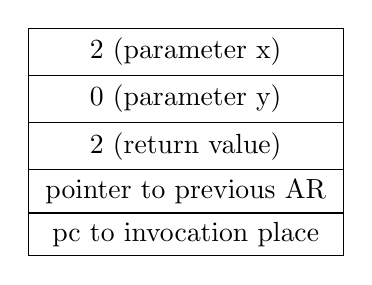
\begin{tikzpicture}
    \node[draw, rectangle split, rectangle split parts=4, 
          minimum width=4cm] at (0,0)
    {
      2  (parameter x) \nodepart{second} 0 (parameter y)
      \nodepart{third} 2 (return value) \nodepart{fourth} pointer to
      previous AR 
    };
    \node[draw, rectangle, minimum width=4cm] at (0,-1.44) 
                                       {pc to invocation place};
  \end{tikzpicture}
\end{enumerate}
}


\newpage
\section{Object-Oriented Programming} \marginpar{\large\textbf{[15 points]}}

\subsection{General}

\begin{enumerate}
\item \comment{\textbf{[1 point]}} Which OO-principle gets easily
  violated when providing setter and getter methods for each field? 
\item \comment{\textbf{[2 points]}} Let \texttt{Person} be a
  Smalltalk class defining the following methods \texttt{m} and
  \texttt{n}
\begin{lstlisting}
Person>>m: aPerson	
  ^aPerson
Person>>n: aPerson	
  ^aPerson
\end{lstlisting}
Consider the following code snippet:
\begin{lstlisting}
|p1 p2| 
p1:=Person new.
p2:=Person new.

(p1 m: p2) n: nil.       (*a*) 
p1 m: p2; n:nil          (*b*)
\end{lstlisting}
Which objects \lstinline!p1! or \lstinline!p2! are the receivers for the
messages \lstinline!m! and \lstinline!n! in \lstinline!(*a*)! and
\lstinline!(*b*)!? \newpage



\item \comment{\textbf{[3 points]}} Given the following class
  hierarchy \\
\begin{center}
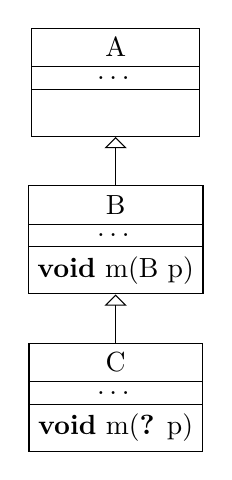
\begin{tikzpicture}
\node[draw, 
   rectangle split, 
   rectangle split parts=3, 
   minimum width=2cm] (A) at (5,4) 
  {A 
     \nodepart{second} \ldots 
     \nodepart{third} \phantom{\textbf{void} h(A x)}};
\node[draw, 
   rectangle split, 
   rectangle split parts=3, 
   minimum width=2cm] (B) at (5,2) 
  {B 
     \nodepart{second} \ldots 
     \nodepart{third} \textbf{void} m(B p)};
\node[draw, 
   rectangle split, 
   rectangle split parts=3, 
   minimum width=2cm] (C) at (5,0) 
  {C 
    \nodepart{second} \ldots 
    \nodepart{third} \textbf{void} m(\textbf{?} p)};   

\draw[open triangle 90-] (A) -- (B);
\draw[open triangle 90-] (B) -- (C);
\end{tikzpicture}
\end{center}
defining all available classes. 
Give for each of the following overriding semantics (for arguments):
\begin{enumerate}
  \item co-variance,
  \item contra-variance and
  \item invariance
\end{enumerate}
all possible argument types for method \lstinline!m! in class
\lstinline!C! such that \lstinline!m! overrides the method
\lstinline!m! declared in class \lstinline!B!. 
\item \comment{\textbf{ [2 points]}} Which of the overriding
  semantics mentioned in the previous item is \emph{not} safe with
  respect to Liskov's (substitution) principle (if you do not know the
  name give a \emph{short} definition of the semantics you mean)?
  Provide an implementation of the method
\begin{center}
\begin{lstlisting}[language=Java, columns=flexible]
void f(A a1, A a2, B b1, B b2, C c1, C c2) { ... }        
\end{lstlisting}
\end{center}
declared in class A consisting of maximal 3 statements exhibiting the
unsafe behavior.

\item Consider the following code snippet
\begin{lstlisting}[language=Java, columns=flexible]
void execute(int cmd, Object[] args) {
  if (cmd == CommandIndex.MOV) { 
         // do move with args 
  } else if (cmd == CommandIndex.ADD) {
         // do add with args
  } else if (cmd == CommandIndex.JMP) {
         // do jump with args
  }
}
\end{lstlisting}
which realises a simple interpreter. 
\begin{enumerate}
\item \comment{\textbf{[1 point]}} The shown solution is not optimal
  as adding new commands requires to change existing code. Which OO
  oriented feature allows a solution that avoids this problem?
 \item \comment{\textbf{[3 points]}} Describe in \emph{at most} 3
   \emph{short} sentences (or draw a UML diagram) the OO solution. 
\end{enumerate}

\end{enumerate}


\solution{
\begin{enumerate}
  \item data encapsulation
  \item (*a*): \texttt{m}: p1 and \texttt{n}: p2\\
        (*b*): \texttt{m}: p1 and \texttt{n}: p1 
  \item \begin{enumerate}
           \item B, C
           \item B, A
           \item B
        \end{enumerate}
  \item co-variance; f(...) { b1.m(b2); }
  \item \begin{enumerate}
    \item dynamic method dispatch
    \item Introduce an (abstract) class \lstinline[language=Java,
      columns=flexible]{Command} declaring an (abstract) method
      \lstinline[language=Java, columns=flexible]{exec(Object[] args)}.
      Subclass the class for each command and implement the body
      accordingly. 
    \end{enumerate}
\end{enumerate}
}

\subsection{F\#}

\begin{enumerate}
  \item \comment{\textbf{[2 points]}}Which of the following statements are true\\
    \begin{tabular}{|p{6cm}|c|c|}\hline
      & True & False \\ \hline
     a) F\# supports classes, but their fields must be immutable & & \\\hline
     b) Mutable variables in F\# are always passed by reference & & \\\hline
     c) One concession of F\#  to the underlying \textsf{.net}
     framework is that types cannot at all be inferred automatically & & \\\hline
     d) F\# supports multiple inheritance of classes & & \\\hline
   \end{tabular}\\
   For your answer draw that table but refer to the statements by a),
   b) etc. instead of writing them again. Wrong answers lead to a
   reduction of points, a negative result does not carry over to other
   sub-assignments. 
 \item \comment{\textbf{[1 point]}} Assume you have two interfaces in F\# named
   \lstinline[language=FSharp]{IPv4} and
   \lstinline[language=FSharp]{IPv6} both declare a method
   \lstinline[language=FSharp]{GetAddress()} which returns the IPv4
   resp.\ IPv6 address. Both kinds of addresses are not compatible. In
   Java this would lead to a problem when a class implements both
   interfaces as no single implementation can cover both
   semantics. Why does F\# not have this kind of problem?
\end{enumerate}

\solution{
\begin{enumerate}
\item 
    \begin{tabular}{|p{6cm}|c|c|}\hline
      & True & False \\ \hline
     a) F\# supports classes, but their fields must be immutable & & X \\\hline
     b) Mutable variables in F\# are always passed by reference & & X \\\hline
     c) One concession of F\#  to the underlying \textsf{.net}
     framework is that types cannot be inferred automatically at all &
     & X \\\hline
     d) F\# supports multiple inheritance of classes & & X\\\hline
   \end{tabular}\\
\item interface methods cannot be called on class types an upcast is
  needed; upcast to different interface types can access idfferent
  methods of same name and signature.
\end{enumerate}

}

\end{document}
